\documentclass{article}

% imports
\usepackage{xcolor}                   % colorize text
\usepackage{graphicx}                 % images
\usepackage{hyperref}                 % hyperlinks
\usepackage[nottoc,numbib]{tocbibind} % include bibliography in toc
\usepackage{wrapfig}                  % wrapped figures
\usepackage{glossaries}               % optional glossary
\usepackage{lipsum}                   % easy lorem ipsum
\usepackage[figurename=Bild]{caption} % rename Figures to Bilder
% overrides & setup
\renewcommand{\refname}{Quellen}
\renewcommand{\contentsname}{Inhaltsverzeichnis}
\graphicspath{{./images/}}
\hypersetup{
    colorlinks=true,
    linkcolor=black,
    citecolor=black,
    filecolor=cyan,
    urlcolor=cyan,
}

\begin{document}
    \begin{titlepage}
        \begin{center}
            \Huge
            \textbf{Solarzellen}

            \vspace{0.5cm}

            \LARGE
            Funktion und Stand der Technik bei Stand-Alone-Anlagen

            \vspace{1.5cm}

            \href{mailto:erik.buennig@fh-erfurt.de}{
                \color{black}{
                    \textbf{Erik Bünnig}
                }
            }\\
            18.2.2021

            \vfill

            \Large
            Projektarbeit zur alternativen Prüfungsleistung im Kurs Elektrotechnik

            \vspace{1.5cm}

            \href{https://www.fh-erfurt.de/fhe/}{
                
\includegraphics[scale=0.5]{fhe_logo}
            }
        \end{center}
    \end{titlepage}

    \tableofcontents
    \thispagestyle{empty}
    \newpage

    \pagenumbering{arabic}

    \section{Vorwort}
        Links (in \textcolor{cyan}{cyan}) und Referenzen (als [\textit{n}]
        dargestellt) beinhalten \textit{hyper links} oder \textit{hyper references}
        zu ihren jeweiligen Herkünften um das Navigieren einfacher zu machen.
        Zusätzlich sind alle Sektionen im Inhaltsverzeichnis ebenfalls verlinkt.
        Diese Arbeit wurde mit \LaTeX{} erstellt, eine Variante mit angenehmeren
        Farben für Lesen bei Dunkelheit ist bereitgestellt.

    \section{Einleitung}
    \subsection{Begrifflichkeiten}
    \subsubsection{Photovoelektrischer Effekt}
        Wechselwirkung von Photonen mit baryonischer Materie, getrennt in
        inneren und äußeren photovoelektrischen Effekt und die Photoionisation.
        \cite{Wiki_PhotoelectricEffect}
    \subsubsection{Photovoltaischer Effekt}
        Sonderfall des inneren photoelektrischen Effekts, beschreibt Bildung eines
        Photostroms, also Trennung von Ladungsträgerpaaren an der p-n-Schicht
        einer Photodiode entgegen der Durchlassrichtung des Übergangs als Folge
        von elektromagnetischer Strahlung auf eine Photodiode.
        Der photovolatische Effekt baut auf der Photoleitung auf, einem weitern
        innerem photoelektrischen Effekt. \cite{Wiki_PhotoelectricEffect}
        Der photovoltaische Effekt dient als Grundlage für die Funktionsweise
        von Solarzellen.
    \subsubsection{Photovoltaischer Zelle}
        Elektrisches Bauelement das auf Grundlage des photvoltaischen Effekts,
Strom erzeugt und aus Halbleitermaterialien (vorwiegend Silizium) besteht.

\subsection{Historie}
    \subsubsection{Entdeckung}
        Die Effekte der Photovoltaik wurden erstmals in 1839 von Andre Edmond
        Becquerel entdeckt, aber erst weit später praktisch angewendet.
        \cite{Wiki_PhotovoltaicHistory}
    \subsubsection{Nennenswerte Ereignisse}
        \begin{itemize}
            \item 1876 - Beweis der direkten Konversion von elektromagnetischer
                Strahlung in elektrische Energie durch William Grylls Adams und
                Richard Evans Day
            \item 1907 - Theoretische Erklärung des photoelektrischen Effekts auf
                Basis der Lichtquantenhypothese (1905) durch Albert Einstein
            \item 1912 - 1916 - Experimentelle Bestätigung von Einsteins Erklärung
                durch Robert Adndrews Millikan
            \item 1958 - Erste Verwendung von Solarzellen zur Versorgung eines
                Satelliten der NASA (Vanguard I) \cite{Wiki_Vanguard}
        \end{itemize}
    \subsubsection{Zukunft}
    % \lipsum[2]
    % \begin{wrapfigure}{l}{0.25\textwidth}
    %     \centering
    %     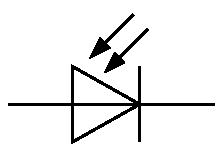
\includegraphics[scale=0.75]{photodiode_symbol.pdf}
    %     \caption{Symbol einer Photodiode \cite{Wiki_Img_PhotodiodeSymbol}}
    % \end{wrapfigure}
    % \lipsum[1]

    \section{Anwendungsgebiete}
    \subsection{IoT-Sensoren}
    Solarzellen eignen sich hervorragend zur Energieversorgung für
    vorwiegend bedienungsfreie Applikationen wie eigenständige
    Sensoren (z.B.: Wetterstation, Luft- oder Wasserqualitätssensoren),
    da diese oft einen geringen stetigen Energieverbrauch aufweisen,
    welcher bei Nacht oder schlechten Wetterverhältnissen mit einer
    Batterie überbrückt werden kann.

\subsection{Weltraum}
    Auch für die Stromversorgung von Satelliten oder Raumstationen
    eignen siche Solarzellen hervorragend, da im Vakuum das auffangen
    elektromagnetischer Strahlung nicht durch atmosphärische Effekte
    behindert.

\subsection{Alternative zu fossilen Brennstoffen}
    \subsubsection{Deutschland}
        In Deutschland wird Solarenergie seit 2000 zunehmend Ausgebaut
        und staatlich gefördert, von 2000 bis 2011 stieg der
        Solarenergieanteil von 64GWh auf 19TWh
        \cite{Wiki_PhotovoltaicGermany}.

    \subsubsection{Kalifornien, USA}
        Der US-Bundesstaat Kalifornien beitet ein gutes Besipiel für
        sowohl Vorteile als auch Nachteile von Solarenergie. In
        hinreichend sonnigen Regionen wie Kalifornien reicht die
        durschnittliche durch Solar produzierte Energie zum Decken des
        durschnittlichen Energieverbrauchs aus. Allerdings sind sowohl
        Produktion als auch Verbrauch von Energie nicht konstant.
        Solaranlagen produzieren ihre Energie hauptsächlich zwischen
        7 Uhr und 18 Uhr.
        \begin{figure}[H]
            \centering
            \includegraphics[width=0.9\linewidth]
            {california_supply_2020-08-01.png}
            \caption{Angebot an Energie in Kalifornien, USA, 01.08.2020
                \cite{Img_CaliforniaSupply}
            }
        \end{figure}
        Der tägliche Verbrauch erreicht vorallem um 17 Uhr bis 22 Uhr
        Höchstwerte. Nächte und Schlechtwettertage müssen dann durch
        gespeicherte, importierte oder lokale nicht-Solarenergie überbrückt
        werden, trotz der großartigen Vorraussetzungen für Solarenergie.
        \cite{SolarCalifornia, YouTube_RE-California}
        \begin{figure}[H]
            \centering
            \includegraphics[width=0.9\linewidth]
            {california_demand_2020-08-01.png}
            \caption{Nachfrage an Energie in Kalifornien, USA, 01.08.2020
                \cite{Img_CaliforniaDemand}
            }
        \end{figure}

    \section{Grundlegender Aufbau und Funktionsweise}
        % TODO
        \subsection{Aufbau}
        \subsection{Funktionsweise}
        \subsection{Effizienz}

    \section{Anwendungsbeispiel}
        % IoT-Sensor 1..2W betrieb durch solarzelle
        % solar zellentyp, größe, kapazität, dunkelheits überbrückung
        \subsection{Problemstellung}
            Gegeben sei eine Wetterstation in einem abgelegenen Teil der Sahara,
            welche zwischen 1W und 2W verbraucht. Wie kann eine solche Anlagen
            kostengünstig und relativ wartungsfrei betrieben werden?
        \subsection{Entwurf}
        \subsection{Konklusion}

    \section{Zusammenfassung}

    \newpage
\begin{thebibliography}{9}
    % Articles
    \bibitem{Wiki_SolarCell}
        \href{https://de.wikipedia.org/wiki/Solarzelle}{
            Wikipedia: Solarzelle
        }\\
        \href{https://en.wikipedia.org/wiki/Solar_cell}{
            Wikipedia: Solarcell (Englisch)
        }

    \bibitem{Wiki_PhotoelectricEffect}
        \href{https://de.wikipedia.org/wiki/Photoelektrischer_Effekt}{
            Wikipedia: Photoelektrischer Effekt
        }

    \bibitem{Wiki_PhotovoltaicHistory}
        \href{https://de.wikipedia.org/wiki/Geschichte_der_Photovoltaik}{
            Wikipedia: Geschichte der Photovoltaik
        }

    \bibitem{Wiki_Vanguard}
        \href{https://de.wikipedia.org/wiki/Vanguard-Projekt}{
            Wikipedia: Vanguard-Projekt
        }

    % Images
    \bibitem{Wiki_Img_PhotodiodeSymbol}
        \href{https://de.wikipedia.org/wiki/Datei:Symbol_Photodiode.svg}{
            Wikipedia: Symbol einer Photodiode
        }

    % Vidoes
    \bibitem{Wiki_Video_RE-SolarFlaw}
        \href{https://www.youtube.com/watch?v=yVOnHWnLSeU}{
            YouTube: Real Engineering - The Mystery Flaw of Solar Panels
        }

    \bibitem{Wiki_Video_RE-California}
        \href{https://www.youtube.com/watch?v=h5cm7HOAqZY}{
            YouTube: Real Engineering - California's Renewable Energy Problem
        }
\end{thebibliography}
\end{document}